\documentclass[fr]{../../../../../../eplexam}

\hypertitle{Théorie des graphes}{5}{INMA}{1961}{2017}{Janvier}{Majeure}
{Etudiants MAP de 2017}
{Vincent Blondel et Jean-Charles Delvenne}

\section{}

\begin{enumerate}
	\item Considérez le graphe de co-présence, qui relie deux personnes si leurs intervalles de présence dans la bibliothèque s’intersectent, et qui est 2-connexe dans notre cas. Démontrez qu’un groupe de personnes forme une clique dans le graphe si et seulement si ces personnes se sont retrouvées ensemble au même moment dans la bibliothèque
	\item Démontrez que l’ensemble des personnes présentes dans la pièce à un moment entre le départ de l’ambassadeur et l’arrivée de son épouse, forme une coupe de noeuds du graphe. Déduisez qu’il y a deux voleurs au minimum, car nul n’aurait pu ouvrir le coffre-fort et le refermer sans se faire remarquer des autres personnes présentes dans la pièce, qui sont dès lors complices. Bien sûr, l’ambassadeur et son épouse sont au-dessus de tout soupçon.
	\item Qui sont les coupables?
	\item Montrez que si un groupe de personnes forme une couverture de sommets alors au moins une des ces personnes est coupable.
	
\end{enumerate}

\begin{figure}[h]
	\centering
	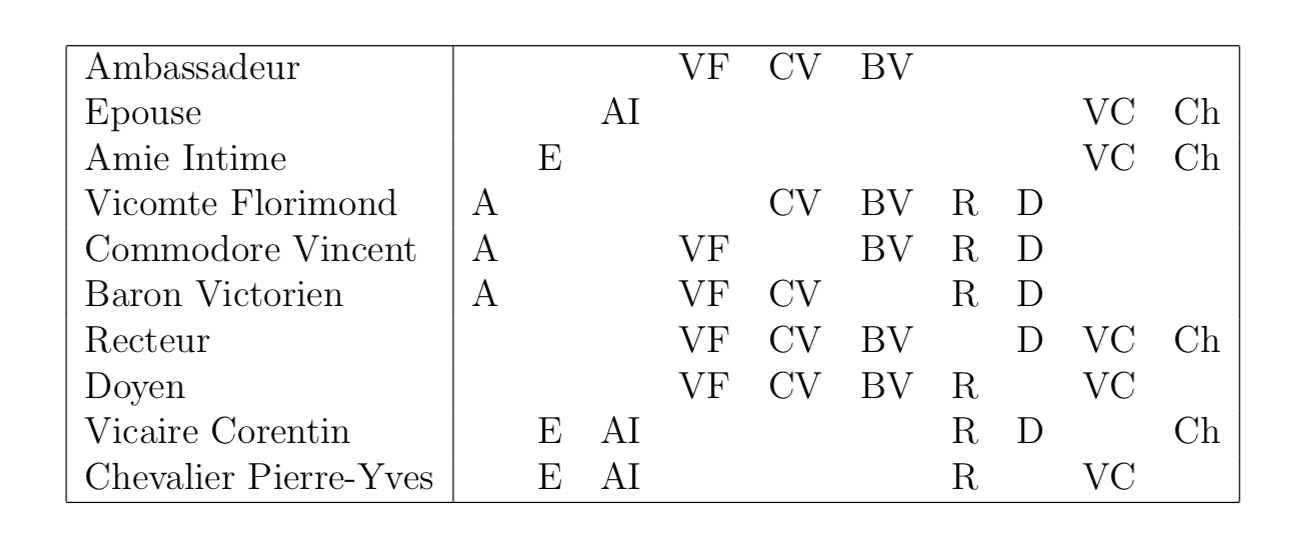
\includegraphics[scale=0.5]{presence.png}
\end{figure}
	
\begin{solution} 
	
\begin{enumerate}
	
	\item Pour chaque personne $i$ correspondant à un noeud de la clique, on définit $a_i=l'h$ d'arrivée et $b_i=d'h$ de départ. Comme les noeuds forment une clique, on a $\forall i,j \quad a_i\leq b_j$ et donc il existe $t$ tel que toutes les personnes de la clique sont présentes en même temps (prendre $\max_i a_i \leq t \leq \min_i b_i$).
		
	\item Une coupe d'un graphe est un ensemble d'arêtes tel qu'il n'y ait plus aucun chemin d'un noeud source vers un noeud puits quand on retire cet ensemble du graphe. Ici le noeud source est l'ambassadeur (qui arrive et part en premier), et le noeud source est l'épouse (qui arrive en dernier).  Donc, l'ensemble des personnes arrivants entre le départ de l'ambassadeur et l'arrivée de l'épouse permet de supprimer tout chemin entre le noeud source et le noeud puits. Pour prouver qu'il y a au minimum 2 voleurs, il faut s'intéresser à la coupe minimum de notre graphe. En visualisant le graphe, nous voyons que R et D sont présents pour 2 groupes de personnes différents. Il suffit donc de prendre comme coupe les arêtes reliant Ch Vc à R et D et nous avons notre coupe minimum.
	
	\item Pour rappel, un set indépendant d'un graphe est un ensemble de sommets qui ne sont pas adjacents entre eux. Le complémentaire de cet ensemble, est appelé la couverture de sommets. 
	
	On a prouvé à la question précédente qu'il existait au moins 2 voleurs, qui étaient donc ensemble dans la bibliothèque pendant le vol, il y a donc une arête qui les relie. Une couverture devant couvrir l'ensemble des arêtes du graphe, et vu qu'il existe une arête entre les 2 (ou plus) voleurs, alors il faut qu'au moins un des voleurs soit dans la couverture

	\item On peut voir que seuls VC et Ch forment une coupe qui ne contient personne de confiance. Ce sont eux les coupables.
	
\end{enumerate}

\end{solution}

\section{}
Emilie, 2 ans, a fait un beau dessin pour son père sur le thème de Noël. Il s’agit d’une courbe fermée.
Cette courbe et ses nombreuses auto-intersections (en nombre fini tout de même) divisent la feuille en un nombre fini de parties. Henri (4 ans) et Guillaume (7 ans) veulent l’enjoliver davantage en coloriant chaque partie de la feuille en bleu ou en rouge, de sorte que deux parties adjacentes (séparées par un arc de courbe) ne soient jamais de la même couleur. Le père se propose de rédiger un question d’examen sur ce thème.
Démontrez ce théorème des deux couleurs : quelle que soit la courbe fermée d’Emilie, ses deux frères pourront réaliser leur dessin.


\begin{solution}
	
On construit un graphe: un noeud = une face sur la courbe, 2 noeuds sont reliés si les faces sont adjacentes. A chaque intersection, on a un nombre pair de chemins qui partent, sinon ce ne serait pas une courbe fermée. A chaque fois qu'on rajoute une intersection, on rajoute une paire de chemi, le graphe total/final n'a pas de cycle de longueur impaire. Donc, il est biparti et ainsi il est 2 coloriable.

\end{solution}

\section{} 

\begin{enumerate}
	\item L’Espagnol veut placer ses troupes en embuscade dans les cols pour réduire au maximum la longueur du front ennemi sans risquer de laisser la route vers Madrid ouverte. Modéliser le problème dans le langage de la théorie des graphes.
	
	\item Résolvez le problème : quels cols (arêtes) sont à défendre ?
	
	\item Si les Français prennent un col aux Espagnols, ceux-ci doivent immédiatement se redéployer de façon à former un nouveau front minimal. Le col à défendre en priorité est donc celui qui donnerait le front le plus difficile à défendre, si pris par les français. Proposez une méthode pour déterminer, dans votre solution, le col à défendre en priorité.
 
	\item Appliquez votre méthode : quel col (arête) est à défendre en priorité ?

\end{enumerate}

\begin{figure}[h]
	\centering
	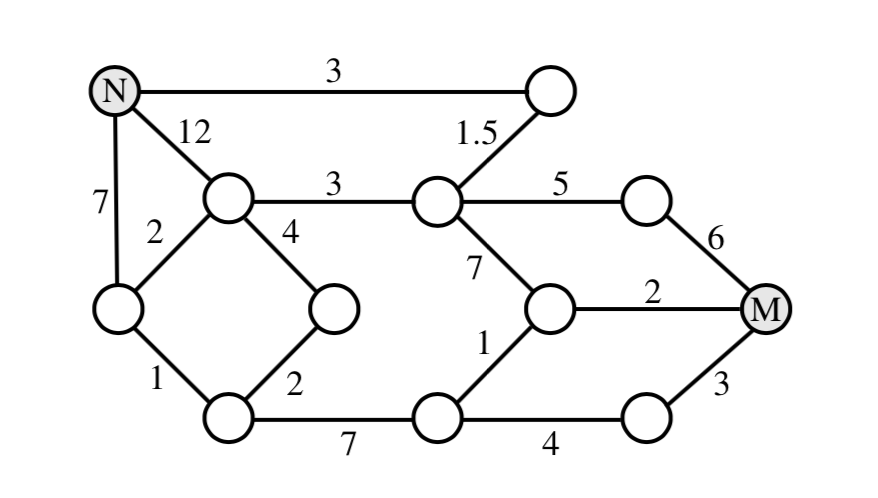
\includegraphics[scale=0.4]{flot.png}
	\caption{relatif à la question 3}
	\label{fig:my_label}
\end{figure}

\begin{solution} 
	
\begin{enumerate}
		
	\item Nous avons un problème de flôt. Le noeud source est les troupe de Napoléon, et le noeud puits est Madrid, le point d'arrivée et l'objectif de ses troupes. L'espagnol veut créer une embuscade afin de réduire au maximum la grandeur du front de Napoléon, chaque route aura alors une capacité dédiée au nombre maximum de troupes qu'elle peut accueillir. Nous essaierons de trouver une coupe minimum afin d'obtenir le flot maximum de ce problème de graphe.
		
	\item En remplaçant l'arête de 3 du dessus par l'arête de 1.5 à côté. Si on fait le flot max on se rend compte qu'il est bien égal à 7.5. Il existe une technique pour récupérer le min-cut une fois qu'on a fait le max flow : tous les noeuds que la source peut encore atteindre via des arêtes non-saturées sont dans S, le reste est dans le complémentaire.
		
	\item Si l'arête (u,v) est prise, on recalcule le min-cut en mettant le noeud v dans S.
		
	\item 
	
\end{enumerate}
	
\end{solution}

\section{Vrai ou faux}

\begin{enumerate}
	
	\item Tout graphe G admettant un couplage parfait est tel que $$\left|\bigcup_{s\in S} \mbox{Voisins}(s)\right| \geq |S|$$ pour tout ensemble de noeuds S.
	
	\item Tout graphe G tel que $|\bigcup_{s\in S} \mbox{Voisins}(s)| \geq |S|$ pour tout ensemble de noeuds S admet un couplage parfait.
	
	\item Tout graphe eulérien connexe est 2-arête-connexe.
	
	\item Tout graphe biparti k-régulier connexe, pour $k > 1$, est 2-arête-connexe.
	
	\item Tout graphe 3-régulier a un nombre pair de noeuds.
	
	\item BONUS. Pour tout coloriage des points du plan en 3 couleurs, il y a deux points de même couleurs séparés par une distance unité (exactement).
	
\end{enumerate}

\begin{solution} 
	
\begin{enumerate}
		
	\item VRAI. Comme il admet un couplage parfait, tout sommet est au moins connecté à un autre via le couplage. Donc, si je considère un ensemble S de sommets comme ils ont tous au moins 1 voisins, l'inégalité est prouvée.
		
	\item FAUX. $K_3$ par exemple.
		
	\item VRAI : C'est un graphe eulérien, il passe par chaque arête 1 et 1 seule fois et forme un cycle. Si on enlève 1 arête, on casse le cycle mais pas la connexité. Il faut enlever 2 arêtes pour la casse.
		
	\item 
		
	\item VRAI. On sait que $\sum \mathrm{deg} = 2\:|\mathrm{arêtes}|$ et donc ici que $3n = 2e$. On peut remarquer que $2e$ sera pair pour toutes les valeurs de $e$. Il faut donc que le produit $3n$ soit pair pour tout $n$. On peut enfin remarquer que c'est le cas pour les valeurs paires de $n$.
		
	\item 
		
\end{enumerate}
	
\end{solution}

\end{document}
